\documentclass[tikz]{standalone}
\usepackage{pgfplots}
\pgfplotsset{compat=1.17}
\usepgfplotslibrary{external}
\usepgfplotslibrary{groupplots}
\usepgfplotslibrary{fillbetween}
\usetikzlibrary{fadings}
\begin{document}
\tikzsetnextfilename{figures/tex/mab-data.pdf}
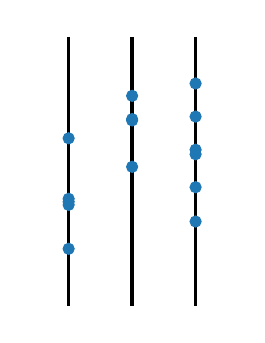
\begin{tikzpicture}
\begin{axis}[axis lines={none}, height={5cm}, width={4cm}, xmin={-1.5}, xmax={1.5}, ymin={-3}, ymax={3}, clip mode={individual}]
    \node at (-1.5,-3) {};
    \node at (1.5,-3) {};
    \node at (1.5,3) {};
    \node at (-1.5,3) {};
    \draw[black, very thick] ({axis cs:-1,0}|-{rel axis cs:0,1}) -- ({axis cs:-1,0}|-{rel axis cs:0,0});
    \draw[black, very thick] ({axis cs:0,0}|-{rel axis cs:0,1}) -- ({axis cs:0,0}|-{rel axis cs:0,0});
    \draw[black, very thick] ({axis cs:1,0}|-{rel axis cs:0,1}) -- ({axis cs:1,0}|-{rel axis cs:0,0});
    \addplot[only marks, color={rgb,1:red,0.1216;green,0.4667;blue,0.7059}]
        coordinates {
            (-1.0,0.7396206598864331)
            (-1.0,-0.7445071021408705)
            (-1.0,-0.6085075626113596)
            (-1.0,-1.7234565107957984)
            (-1.0,-0.6756156074023714)
        }
        ;
    \addplot[only marks, color={rgb,1:red,0.1216;green,0.4667;blue,0.7059}]
        coordinates {
            (0.0,1.167484750027598)
            (0.0,0.10381164512481122)
            (0.0,1.1385638307985484)
            (0.0,1.68617235607297)
        }
        ;
    \addplot[only marks, color={rgb,1:red,0.1216;green,0.4667;blue,0.7059}]
        coordinates {
            (1.0,1.9613911936905772)
            (1.0,0.38372765017046945)
            (1.0,-1.115504071589022)
            (1.0,0.4851584297344153)
            (1.0,1.223914307080334)
            (1.0,-0.3503890587311874)
        }
        ;
\end{axis}
\end{tikzpicture}
\end{document}
